\section{Introduction to Machine Learning}
\begin{flushleft}
    \large Machine Learning (ML) is a powerful subset of artificial intelligence (AI) that empowers computers to learn from data and make predictions or decisions without the need for explicit programming. Rather than following static, rule-based instructions, machine learning models identify patterns, structures, and relationships within data. These models generalize from known data to make predictions about new, unseen data, much like how humans learn from past experiences. \break
    
    Consider the task of recognizing handwritten digits, like those in postal addresses or bank checks. We can train a machine learning model using a dataset of labeled images, where each image corresponds to a digit from 0 to 9. The model learns to recognize the unique patterns of each digit by analyzing features such as curves, edges, and line intersections. Over time, the model refines its ability to correctly identify digits it has never encountered before, thus demonstrating its ability to generalize from the data it was trained on.
\end{flushleft}
\subsection{Data Splitting: Train and Test Sets}
\begin{flushleft}
\large \textbf{Train/Test Split} refers to this method of dividing the dataset, typically using an 80-20 or 70-30 ratio. For example, in an 80-20 split, 80\% of the data is used for training, and the remaining 20\% is held back for testing


The reason we need a test set is to prevent \textbf{overfitting}, a common problem where a model becomes too tailored to the training data, performing well on it but poorly on new data. By evaluating on the test set, we can gauge whether the model has generalized well beyond the data it was trained on.

In practice, the following steps are often taken when working with train/test splits:
\begin{itemize}
    \item \textbf{Step 1: Data Splitting.} Split the data into training and test sets before training the model. This prevents any information from the test set from leaking into the model.
    \item \textbf{Step 2: Model Training.} Use the training set to build the machine learning model by adjusting weights, minimizing errors, or finding patterns.
    \item \textbf{Step 3: Model Evaluation.} Once the model is trained, evaluate it on the test set. Common evaluation metrics include accuracy, precision, recall, and mean squared error, depending on the type of model.
\end{itemize}

In some cases, a third subset called a \textbf{validation set} is also used. The validation set helps tune hyperparameters and prevent overfitting before final testing on the test set.

This train/test split method is fundamental to machine learning as it ensures that models can be assessed on their ability to generalize, avoiding bias toward the data they were trained on.
\end{flushleft}
\subsection{Regression and Classification Tasks}
\begin{flushleft}
    \large Machine learning generally tackles two major types of problems: regression and classification. \break
    
    \textbf{Classification} is the task of categorizing a set of items into predefined classes. For example, classifying an image as either a “cat” or a “dog.” The output is typically a discrete label, such as “yes” or “no,” or in this case, “cat” or “pig.” \break
    
    On the other hand, \textbf{regression} is about predicting a continuous value. For instance, predicting a person’s weight based on their height is a regression task, where height is the input feature and weight is the predicted continuous value. In multiple regression, multiple features (like height, age, etc.) are used to predict an output, such as house prices or stock market trends.
\end{flushleft}

\section{Linear Regression: Regression}
\subsection{Fundamentals of Linear Regression}
\begin{flushleft}
    \large In machine learning, linear regression is one of the most fundamental algorithms. It tries to model the relationship between input features and the target output by fitting a straight line to the data points. The general form of a linear regression model is:
        $$\hat{y} = b + w_1x_1 + w_2x_2 + ... + w_nx_n$$
    Where:
    \begin{itemize}
        \item \( \hat{y} \) is the predicted output,
        \item \( x_1, x_2, ..., x_n \) are the input features,
        \item \( w_1, w_2, ..., w_n \) are the weights (coefficients) assigned to each feature,
        \item \( b \) is the intercept.
    \end{itemize}
    The goal of linear regression is to find the values of \( w \) and \( b \) that minimize the difference between the predicted values and the actual target values in the training data. This is often done by minimizing the Sum of Squared Errors (SSE).
\end{flushleft}
\subsection{Understanding Sum of Squared Errors (SSE)}
\begin{flushleft}
    \large The \textbf{Sum of Squared Errors (SSE)} is a commonly used metric in regression analysis to quantify how well a model fits the observed data. It measures the total difference (or error) between the actual values (from the dataset) and the predicted values (generated by the model). Specifically, SSE sums the squared differences between each actual value and its corresponding predicted value. By squaring these differences, the metric ensures that all deviations are counted positively (i.e., large errors in either direction, above or below, contribute significantly to the total error).

    The formula for SSE is:
    \begin{center}
        \( SSE = \sum_{i=1}^{m} (y_i - \hat{y}_i)^2 \)
    \end{center}
    
    Where:
    \begin{itemize}
        \item \( y_i \) represents the \textbf{actual value} for data point \( i \),
        \item \( \hat{y}_i \) represents the \textbf{predicted value} from the model for the same data point,
        \item \( m \) is the \textbf{number of data points} in the dataset.
    \end{itemize}

    The concept of squaring the errors is essential because it penalizes larger deviations more than smaller ones. In other words, if a prediction is far off from the actual value, its contribution to the SSE will be disproportionately larger, making it easier to identify large errors. \break

    \begin{figure}[H]
        \centering
        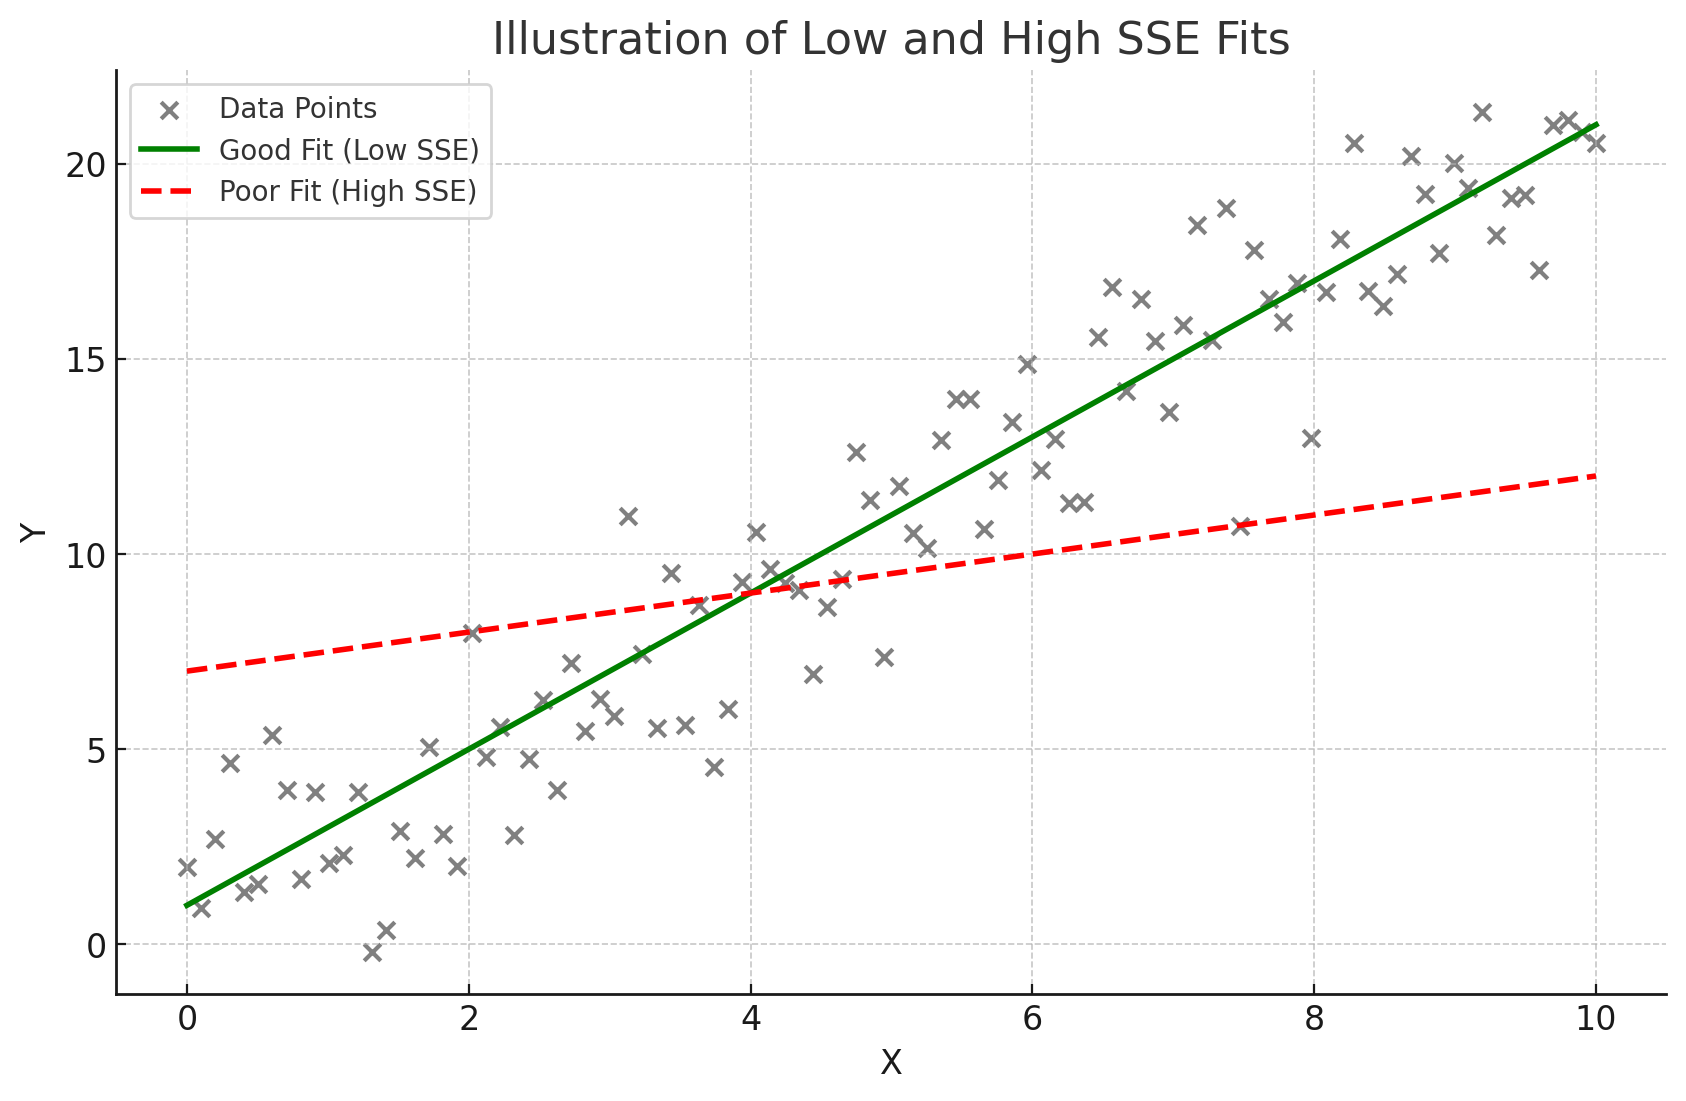
\includegraphics[width=0.45\linewidth]{ml/seefits.png}
        \caption{An illustration of two lines of fit that would produce a low and high SSE respectively. The line that fits the data better has a low SSE}
        \label{fig:seefits}
    \end{figure}

    \textbf{The goal in regression} is to minimize SSE, because a lower SSE value indicates a better fit of the model to the data. A model with a small SSE suggests that its predictions are close to the actual observed values, indicating that the model is accurate and effectively capturing the patterns in the data.
\end{flushleft}
\subsection{Minimizing SSE: Simple Case}
\begin{flushleft}
    \large \textbf{Least Squares Regression} is one of the most widely used methods in statistics for finding the best-fitting line through a set of data points. The term “least squares” refers to the fact that the method seeks to minimize the \textbf{sum of squared differences} (i.e., the SSE) between the observed values and the values predicted by the regression line. The result is a line (or, in higher dimensions, a hyperplane) that minimizes the overall prediction error across all data points.

    In simple linear regression, the model is expressed as:
    \begin{center}
        \( \hat{y} = w_0 + w_1x \)
    \end{center}
    Where:
    \begin{itemize}
        \item \( w_0 \) is the \textbf{intercept} of the line, representing the predicted value when the input \( x = 0 \),
        \item \( w_1 \) is the \textbf{slope} or weight, representing the change in the predicted value \( \hat{y} \) for a one-unit change in the input \( x \),
        \item \( x \) is the input (or feature) variable, and
        \item \( \hat{y} \) is the predicted value based on the input.
    \end{itemize}

    In the least squares method, the goal is to find the optimal values for \( w_0 \) and \( w_1 \) that minimize the SSE, ensuring that the line fits the data as closely as possible. The same concept can be extended to multiple regression, where we aim to minimize the SSE by adjusting multiple weights \( w_1, w_2, ..., w_n \).

    Mathematically, this optimization process requires taking the partial derivatives of SSE with respect to the weights (including the intercept) and setting them to zero. This gives us the \textbf{normal equations}:
    \begin{center}
        \( w_0 = \frac{\sum y - w_1\sum x}{n} \)
    \end{center}
    \begin{center}
        \( w_1 = \frac{\sum(x_i - \bar{x})(y_i - \bar{y})}{\sum(x_i - \bar{x})^2} \)
    \end{center}

    These equations provide the values of the intercept (\( w_0 \)) and the slope (\( w_1 \)) that minimize SSE. Once these values are calculated, the resulting regression line represents the best-fitting line for the data according to the least squares criterion.
\end{flushleft}
\subsection{Minimizing SSE: General Case}
\begin{flushleft}
    \large What if you had a model with many more input features, like the one we showed at the beginning of the article?

    $$\hat{y} = b + w_1x_1 + w_2x_2 + ... + w_nx_n$$

    It becomes much easier to represent the solution for the weights in matrix form. However, we need to translate what we have here into matrix form first. \break 
    
    We first define $\textbf{w}$ as a vector consisting of all the weights in our model:

    $$\textbf{w} = \begin{bmatrix}
            w_1\\
            w_2\\
            \vdots\\
            w_n\\
            \end{bmatrix}$$

    Our goal is to find $\hat{\textbf{w}}$, the weights for our model that minimize the SSE. Similarly, we define $\textbf{x}_i$ as a vector consisting of all the features \textit{of a single datapoint}:

    $$\textbf{x}_i = \begin{bmatrix}
            x_1\\
            x_2\\
            \vdots\\
            x_n\\
            \end{bmatrix}$$

    You can think of each $\textbf{x}_i$ as a point in n-dimensional space. We denote this mathematically as $\textbf{x}_i \in \mathbb{R}^n$. Using this, we can define $X$ as a matrix holding all of our $m$ datapoints:

    $$X = \begin{bmatrix}
            \textbf{x}_1^{\top}\\
            \textbf{x}_2^{\top}\\
            \vdots\\
            \textbf{x}_m^{\top}\\
            \end{bmatrix}$$

    We say that $X \in \mathbb{R}^{m \times n}$. Finally, we define $\textbf{y}$ as a vector holding all of our true labels $y$ from our training set.

    $$\textbf{y} = \begin{bmatrix}
            y_1\\
            y_2\\
            \vdots\\
            y_m\\
            \end{bmatrix}$$

    The amount of $y$ values is the same as the amount of $x$ points ($m$). Using these elements, we can actually very easily construct a closed-form solution to $\hat{\textbf{w}}$!

    $$\hat{\textbf{w}} = (X^{\top}X)^{-1}X^{\top}\textbf{y}$$

    How to derive this is a tad beyond the scope of this article, especially if you are unfamiliar with matrix calculus. However, the proof is provided below for thoroughness. For a quick refresher on matrix algebra, see \href{https://www.youtube.com/playlist?list=PLZHQObOWTQDNU6R1_67000Dx_ZCJB-3pi}{Essence of Linear Algebra Series by 3Blue1Brown}. For a quick refresher on matrix calculus, see \href{https://www.youtube.com/watch?v=tIkzL4jlt8g}{Matrix Calculus for Machine Learning by StatQuest}.
 
    \begin{align*}
        \hat{\textbf{w}} &= \argmin_w \sum_{i=1}^n (y_i - \hat{y}_i)^2 && \text{Find $\textbf{w}$ that minimizes the SSE. This is $\hat{\textbf{w}}$.}\\
        &= \argmin_w \sum_{i=1}^n (y_i - (\textbf{x}_i^{\top}\textbf{w} + b))^2 && \text{Plug in $\hat{y}_i = \textbf{x}_i^{\top}\textbf{w} + b$.}\\
        &= \argmin_w \sum_{i=1}^n (y_i - (\textbf{x}_i^{\top}\textbf{w}))^2 && \text{\parbox{0.5\textwidth}{Disregard $b$, since an intercept can be represented by appending a 1 to $\textbf{x}$.}}\\
        0 &= \frac{\partial}{\partial w} \sum_{i=1}^n (y_i - (\textbf{x}_i^{\top}\hat{\textbf{w}}))^2 && \text{\parbox{0.5\textwidth}{Find $\hat{\textbf{w}}$ by taking the partial derivative of the argmin term and setting it equal to 0.}}\\
        &= \sum_{i=1}^n \frac{\partial}{\partial w} (y_i - (\textbf{x}_i^{\top}\hat{\textbf{w}}))^2 && \text{Property of derivatives.}\\
        &= \sum_{i=1}^n 2(y_i - \textbf{x}_i^{\top}\hat{\textbf{w}})(-\textbf{x}_i) && \text{Derive.}\\
        &= \sum_{i=1}^n (y_i - \textbf{x}_i^{\top}\hat{\textbf{w}})(
        \textbf{x}_i) && \text{Divide by -2}\\
        &= \sum_{i=1}^n (
        \textbf{x}_i)(y_i - \textbf{x}_i^{\top}\hat{\textbf{w}}) && \text{The term $y_i - \textbf{x}_i^{\top}\hat{\textbf{w}}$ is a scalar. $c\textbf{x} = \textbf{x}c$}\\
        &= \sum_{i=1}^n (\textbf{x}_iy_i - \textbf{x}_i\textbf{x}_i^{\top}\hat{\textbf{w}}) && \text{Distribute}\\
        &= \sum_{i=1}^n \textbf{x}_iy_i - \sum_{i=1}^n \textbf{x}_i\textbf{x}_i^{\top}\hat{\textbf{w}} && \text{Distribute}\\
        (\sum_{i=1}^n \textbf{x}_i\textbf{x}_i^{\top})\hat{\textbf{w}} &= \sum_{i=1}^n \textbf{x}_iy_i && \text{Move second term to LHS.}\\
        (X^{\top}X)\hat{\textbf{w}} &= X^{\top}\textbf{y} && \text{\parbox{0.5\textwidth}{Convert from vector summation form to matrix form}}\\\\
        (X^{\top}X)^{-1}(X^{\top}X)\hat{\textbf{w}} &= (X^{\top}X)^{-1}X^{\top}\textbf{y} && \text{Left multiply by $(X^{\top}X)^{-1}$}\\
        \hat{\textbf{w}} &= (X^{\top}X)^{-1}X^{\top}\textbf{y} && \text{Cancel}\\
    \end{align*}

    This is pretty amazing. If you were to create just $X$ and $\textbf{y}$ for any regression dataset, you can find $\hat{\textbf{w}}$. It doesn't matter how many features you have, this will work. We also know \textit{for a fact} that these weights in $\hat{\textbf{w}}$ are the weights that will minimize the SSE the most due to a property called \textbf{convexity}. We will come back to what this is later. In addition to linear regression, we have two other very common types of regression called Ridge and LASSO.
\end{flushleft}

\subsection{Ridge and LASSO Regressions}
\begin{flushleft}
    \large We must first quickly introduce a concept called \textbf{regularization}. Quite often, you will find that the weights estimated by $\hat{\textbf{w}}$ do minimize the SSE for training data, but can perform poorly on real-world data post model deployment. This is because the weights found are \textit{too well tuned} to the training data, and cannot generalize with the same performance to unseen data. What can also happen is that some weights will become very large, since the feature they are associated with is important for predicting $y_i$. Let's say we are training a regression model to predict house prices based on house features. One feature could indicate if a house is a lakefront property. Since our training data is primarily from Florida, the indication of a lakefront property means that the property has a very high value. So, the model basically \textit{just} uses this one feature to predict housing price. All other features have their associated weights very low, meaning they barely influence the model's output. The model works just fine for houses in Florida. However, when we go to predict the prices of houses in Wyoming, we see that none of them are lakefront properties and therefore this feature that the model placed so much importance on has become useless. The model ``put all its eggs in one basket'' and now has poor performace on real data despite performing wonderfully on the training set! We will explore this concept further when talking about the \textbf{bias-variance tradeoff}, but for now just understand that the weights you find with ordinary linear regression tend to not generalize well. \break

    \begin{figure}[H]
        \centering
        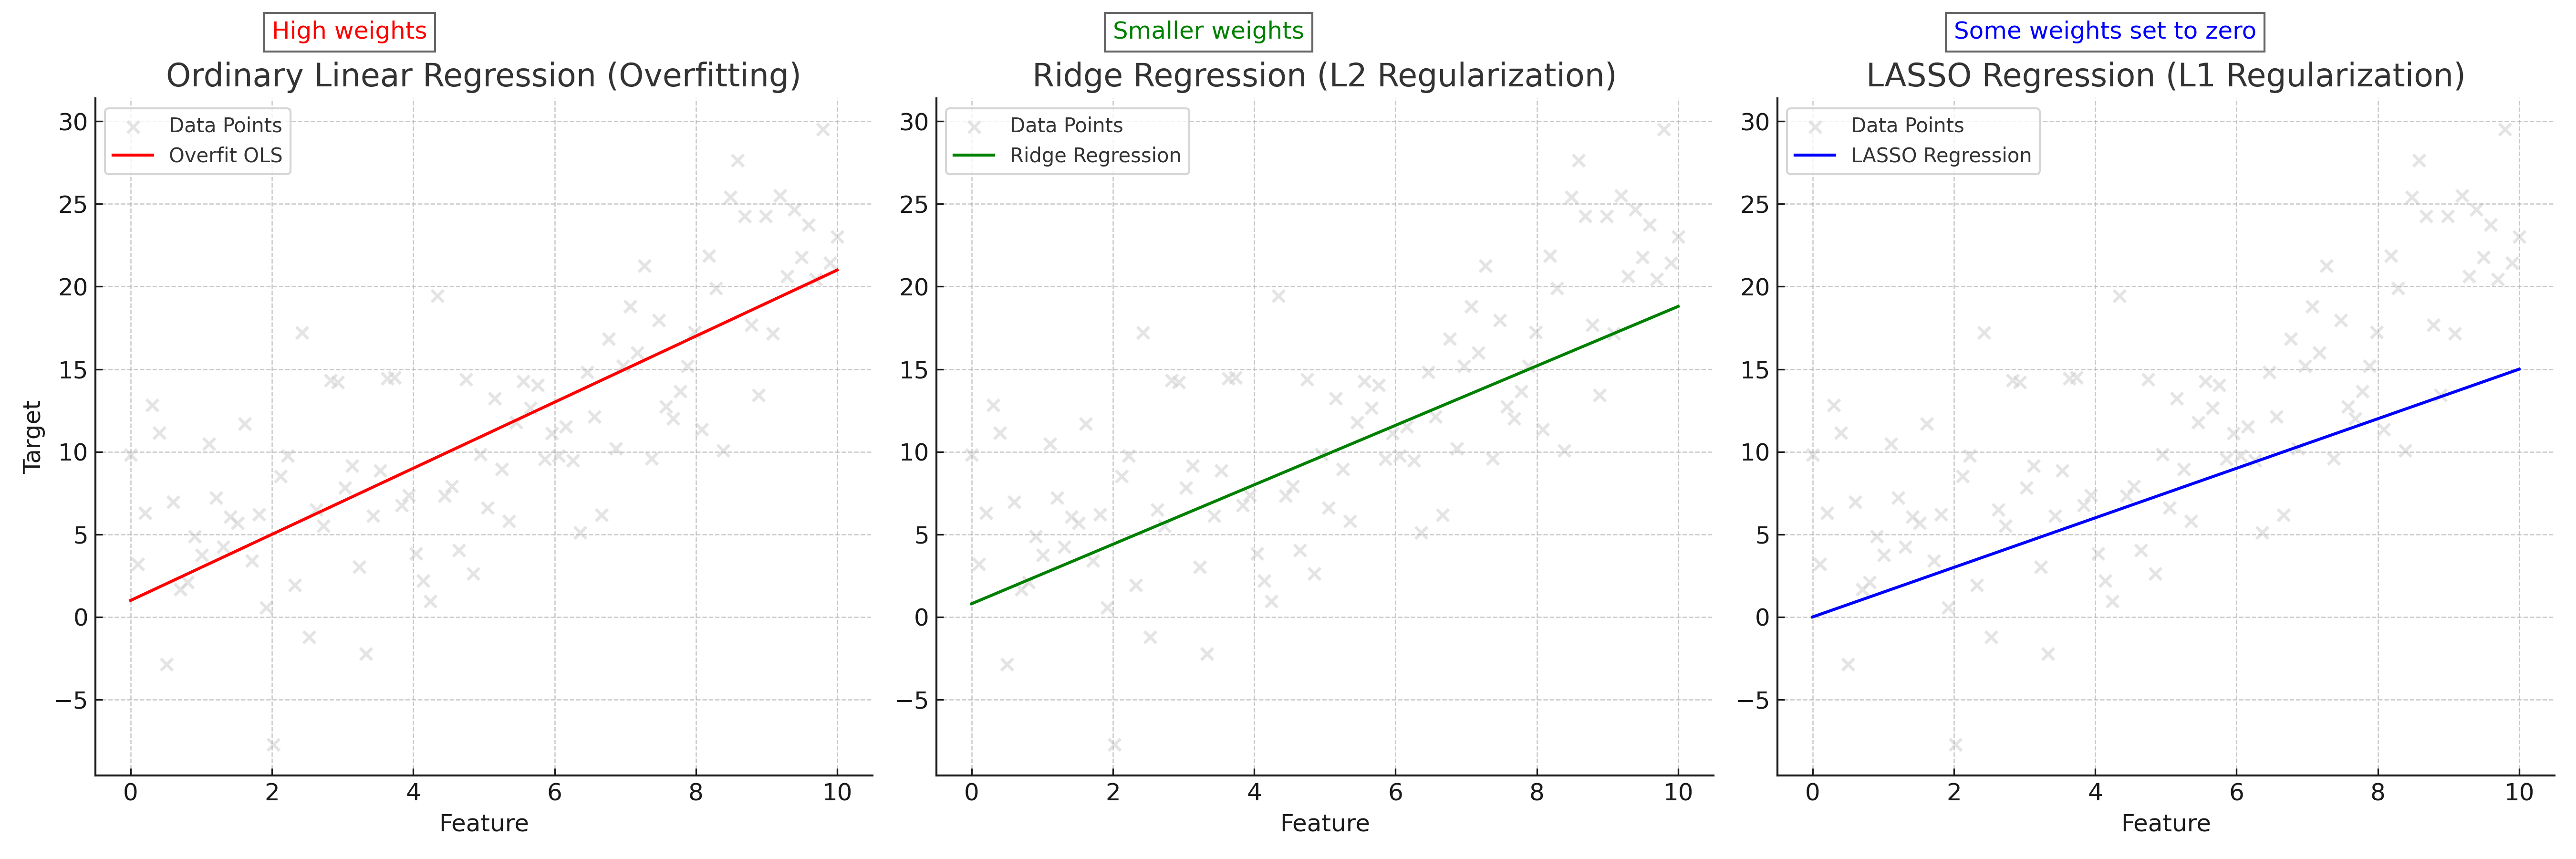
\includegraphics[width=0.85\linewidth]{ml/regression_comparison.png}
        \label{fig:regression_comparison}
    \end{figure}
    
    What can we do in this case? Well, we can penalize weights becoming too high by modifying our SSE optimization objective to include a term that increases as the weights do. This will encourage the model to find a solution for $\hat{\textbf{w}}$ while keeping the weights more balanced. What this term is determines which linear regression variant we get. If we use the L2-norm, we get \textbf{Ridge regression}. If we use the L1-norm, we get \textbf{LASSO} regression. If we use both, we get \textbf{ElasticNet}. This last model is beyond the scope of this article, but we will explore how the first two behave. \break

    But first, what are the L2 and L1 norms? These norms are mathematical functions that map from vector space to scalar space ($\mathbb{R}^n \rightarrow \mathbb{R})$. They are defined as such:

    \begin{align*}
      \|\textbf{x}\|_2 &= \sqrt{\sum_{i=1}^n x_i^2} \\
      \|\textbf{x}\|_1 &= \sum_{i=1}^n \vert x_i \vert
    \end{align*}

    So the L2 norm is the square root of the sum of squared elements from the vector, and the L1 norm is the sum of the absolute value of elements from the vector. These are our regularizers. If we calculate these norms on $\hat{\textbf{w}}$, you can see that the result gets larger if the elements of $\hat{\textbf{w}}$ are large/unbalanced (something we don't want). We want to find a solution that attempts to minimize $||\hat{\textbf{w}}||_2$ or $||\hat{\textbf{w}}||_1$ along with the original SSE objective. We therefore write our two new optimization objectives down:

    \begin{align*}
      Ridge\;SSE &= \sum_{i=1}^{m} (y_i - \hat{y}_i)^2 + \lambda\|\hat{\textbf{w}}\|_2 \\
      LASSO\;SSE &= \sum_{i=1}^{m} (y_i - \hat{y}_i)^2 + \lambda\|\hat{\textbf{w}}\|_1
    \end{align*}

    The $\lambda$ term allows us to control how much regularization we want. A small number makes the mode kind of ``care'' about keeping its weights down. A large value forces the model to keep its weights down at the expense of weights that actually fit the data. Finding the right value for $\lambda$ is a balancing act. \break

    As for how to actually find $\hat{\textbf{w}}$ for these new optimization objectives, that is a little tricky. Ridge regression has a closed-form solution that can be derived similar to ordinary linear regression. It also looks quite similar:

    $$\hat{\textbf{w}} = (X^{\top}X + \lambda I)^{-1}X^{\top}\textbf{y}$$

    $I$ is the identity matrix, a $\mathbb{R}^{n \times n}$ matrix in this case with ones down the diagonal and zeroes everywhere else. How this comes about is hidden in the algebra and calculus of the derivation. That derivation is much beyond the scope of this article, but not impossible to understand if you grasp the ordinary linear regression closed form solution derivation. For LASSO, you have to use more complex techniques like variations of \textbf{gradient descent}. We will cover this topic in later units. \break

    What is the difference between these two linear regression variants? If you use Ridge regression, your final $\hat{\textbf{w}}$ value will have weights that are low and spread out across all features. If you use LASSO regression, you will get a ``sparse'' $\hat{\textbf{w}}$, meaning that unimportant features will have their weights set to 0 and the important ones will have nonzero values. This is due to how the norms manifest on the ``loss landscape''. As shown in Figure \ref{fig:l1_l2}, the solution (minima) to the Ridge SSE or LASSO SSE must sit on the intersection of the a contour (oval) and the shape created by the norm. For L1, this norm has peaks at the axes, causing solutions to have zero values for $w_1$ but nonzero values for $w_2$. The L2 norm is less harsh, with a lower but nonzero value for $w_1$. Cranking up $\lambda$ will exaggerate these effects, with incredibly high values for $\lambda$ in LASSO regression resulting in only one or two features having non-zero weights.

    \begin{figure}[H]
        \centering
        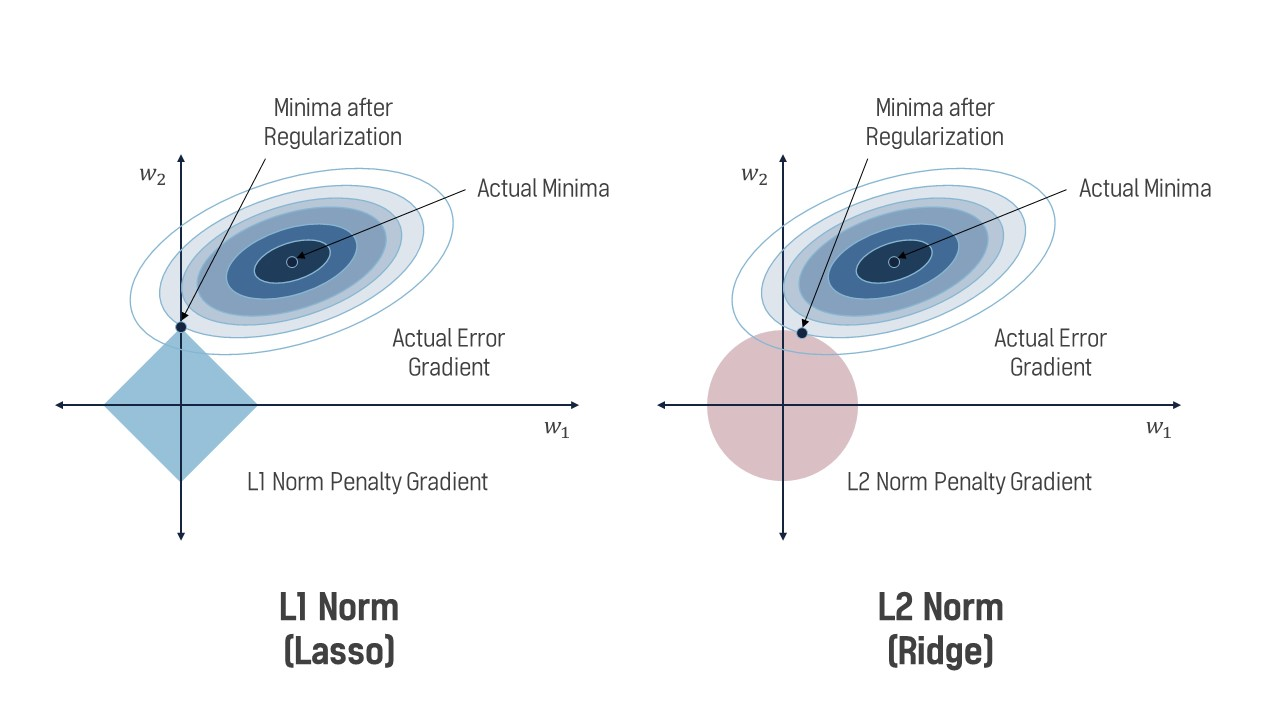
\includegraphics[width=0.9\linewidth]{ml/l1_l2.jpg}
        \caption{Showing how the L1 and L2 norms influence $\hat{\textbf{w}}$ through the nature of their manifestations on the loss landscape as a hyperdiamond and hypersphere respectively}
        \label{fig:l1_l2}
    \end{figure}

    Both of these regression variants have use cases where they shine, so no one is ``better'' than the other. Ridge regression should be used when you want to ensure all features influence the final output, and you should use LASSO when you want to perform intelligent ``feature pruning'' and only use relevant features for the final output (perhaps due to computational constraints).
\end{flushleft}

\begin{questionbox}
\textbf{Synthesis Questions:}
\begin{enumerate}
    \item What is SSE? Why do we want to minimize it?
    \item What do the following symbols represent, and what are their shapes? (Assume $n$ is the dimensionality of the data and $m$ is the number of datapoints):
    \begin{itemize}
        \item $\textbf{w}$
        \item $\hat{\textbf{w}}$
        \item $X$
        \item $\textbf{y}$
    \end{itemize}
    \item Rewrite the euclidean distance formula $d(x,y) = \sqrt{\sum_{i=1}^n (x_i-y_i)^2}$ using the L2-norm $||\textbf{x}||$ given two vectors $\textbf{x}$ and $\textbf{y}$. Do you notice any relationship between the L2-norm and euclidean distance?
    \item In your own words, what are the differences between Ordinary, Ridge, and LASSO regressions?
    \item \textbf{Bonus:} Solve for $\hat{\textbf{w}}$ in the Ridge regression setting. Here is the equation: $$\underset{w}{argmin} \sum_{i=1}^n (y_i - \hat{y}_i)^2 + \lambda||\hat{\textbf{w}}||_2^2$$ Your answer should be the closed form solution for Ridge regression and the proof should be similar to the one given for ordinary linear regression.
\end{enumerate}
\end{questionbox}

\section{Logistic Regression: Classification}
\subsection{Fundamentals of Logistic Regression}
\begin{flushleft}
    \large Logistic regression, despite its name, is a classification algorithm used to predict a binary outcome—often represented as a “yes/no” or “1/0.” Unlike linear regression, which predicts continuous values, logistic regression is designed to output the probability that a given input belongs to a certain class. For instance, it can help us predict if an email is spam or not based on various features.

    The fundamental idea behind logistic regression is to use a \textbf{sigmoid function} to transform the output of a linear equation (a combination of input variables) into a probability between 0 and 1. The probability tells us how likely the input belongs to one of two possible classes, usually denoted as 1 (positive class) or 0 (negative class). The sigmoid function is defined as:

    \begin{center}
        \( P(y=1 \mid x) = \frac{1}{1 + e^{-(b + w^{\top}x)}} \)
    \end{center}
    
    Where:
    \begin{itemize}
        \item \( w \) is the \textbf{weight vector}, which defines the importance of each feature in the input.
        \item \( b \) is the \textbf{bias term}, which adjusts the overall output of the function.
        \item \( e \) is Euler’s number, and the exponent ensures that the output is squeezed between 0 and 1.
    \end{itemize}
\end{flushleft}

\subsection{The Sigmoid Function and Its Role}
\begin{flushleft}
    \begin{figure}[H]
        \centering
        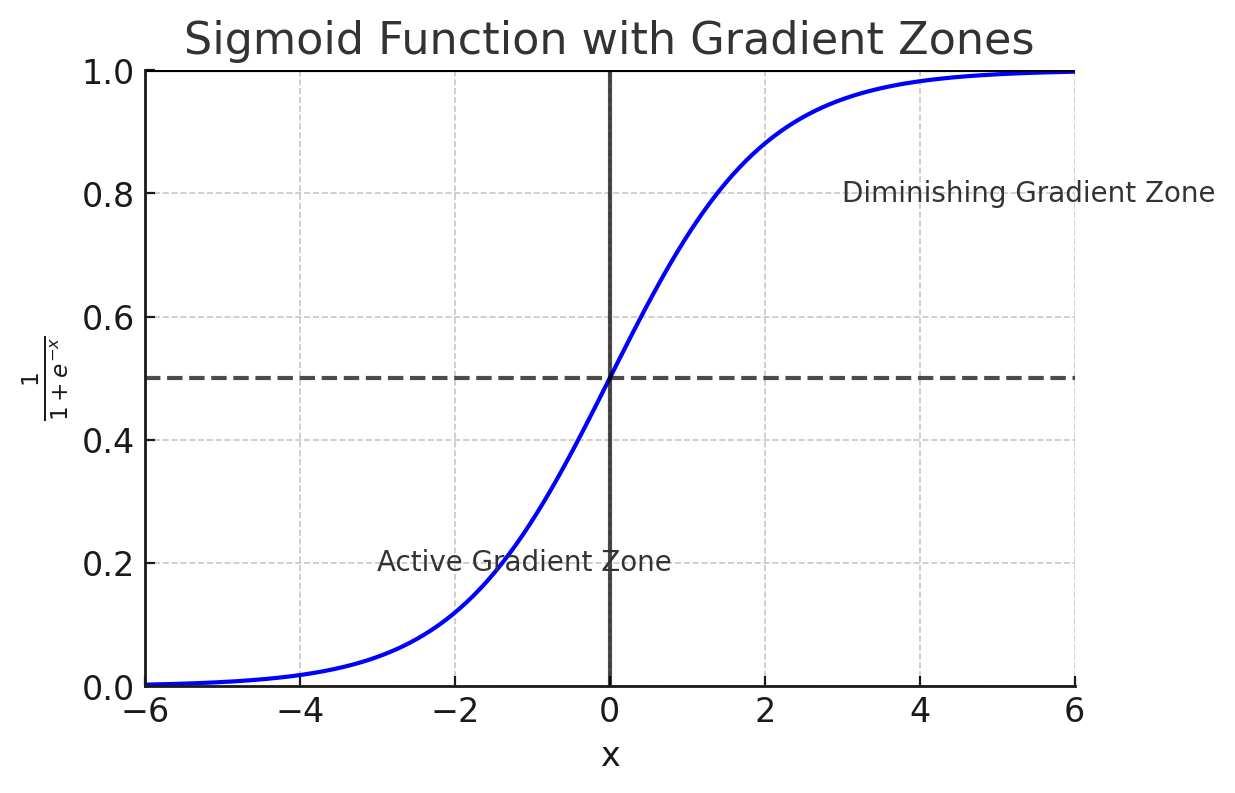
\includegraphics[width=0.45\linewidth]{ml/sigmoid_function.png}
        \caption{A graph showing the sigmoid function.}
        \label{fig:sigmoid_function}
    \end{figure}
    
    \large The sigmoid function plays a crucial role in logistic regression because it takes any input from the linear equation and converts it into a value between 0 and 1. This value can be interpreted as a probability, helping us decide which class the input most likely belongs to. Here's how it works:
    
    \begin{itemize}
        \item If the result of the linear equation (\( b + w^{\top}x \)) is a large positive number, the sigmoid function outputs a value close to 1, indicating that the input most likely belongs to class 1.
        \item If the result is a large negative number, the sigmoid function outputs a value close to 0, indicating class 0.
        \item If the result is near 0, the sigmoid outputs a value close to 0.5, meaning the input is equally likely to belong to either class.
    \end{itemize}
    
    This probability can then be used to classify the input: if the probability is greater than 0.5, we predict class 1, and if it is less than 0.5, we predict class 0.
\end{flushleft}

\subsection{Training with the Log-Likelihood Loss}
\begin{flushleft}
    \large To make logistic regression work effectively, we need to find the best values for the weights \( w \) and bias \( b \). This is done by minimizing the \textbf{log-likelihood loss function}. This function measures how well the model’s predicted probabilities match the actual class labels. By adjusting the weights and bias to minimize this loss, we ensure that the model produces the most accurate predictions.

    During training, the model learns to minimize this loss by using optimization techniques like gradient descent. This ensures that the weights are fine-tuned to give the highest probability for the correct class as often as possible.
\end{flushleft}

\subsection{Extensions to Multiclass Classification}
\begin{flushleft}
    \large While logistic regression is primarily used for binary classification, it can be extended to handle multiple classes through methods such as \textbf{one-vs-rest (OvR)}. In this approach, we train multiple logistic regression models, each one responsible for distinguishing whether an input belongs to one particular class or any of the others. The model with the highest probability ultimately decides the final class label.
\end{flushleft}

\subsection{Why It's Called “Regression”}
\begin{flushleft}
    \large The term ``logistic regression'' comes from its similarity to \textbf{linear regression}. Both methods start by calculating a linear combination of the input features. However, while linear regression outputs continuous values, logistic regression uses the sigmoid function to turn these values into probabilities, which are used for classification tasks. This difference is crucial to understanding why logistic regression is a classification algorithm despite having ``regression'' in its name.
\end{flushleft}

\begin{questionbox}
\textbf{Synthesis Questions:}
\begin{enumerate}
    \item How does the sigmoid function play a role in making Logistic Regression a classification algorithm?
    \item For the algorithm to say that the input is equally likely to be from either class, what must have $b + w^{\top}x$ have been?
\end{enumerate}
\end{questionbox}

\section{K-Means Clustering: Unsupervised Learning}
\subsection{Introduction to Unsupervised Learning}
\begin{flushleft}
    \large In contrast to supervised learning, which learns from labeled data, \textbf{unsupervised learning} operates on \textbf{unlabeled data} and aims to find hidden patterns or structures within it. One powerful method used in unsupervised learning is \textbf{k-means clustering}. This algorithm attempts to group data points into \( k \) clusters, where each cluster contains points that are similar to each other. Unlike supervised methods where there is a clear ``right answer'', the objective here is to let the algorithm uncover these clusters on its own.
\end{flushleft}

\subsection{How K-Means Clustering Works}
\begin{flushleft}
    \large At its core, k-means clustering is about finding the best way to group data points. This process involves iteratively assigning data points to clusters and then recalculating the center of each cluster, known as the \textbf{centroid}. The idea is to minimize the distance between data points and their corresponding centroids, so points within a cluster are more similar to each other than to points in other clusters.

    The process of k-means clustering can be broken down into the following steps:
    \begin{itemize}
        \item \textbf{Step 1: Initialization.} The algorithm begins by randomly selecting \( k \) initial cluster centroids from the dataset. These centroids act as the starting points for the clusters.
        
        \item \textbf{Step 2: Assignment.} Each data point is assigned to the nearest centroid based on a distance metric, typically Euclidean distance. This forms \( k \) clusters of data points, with each point belonging to the cluster whose centroid is closest.
        
        \item \textbf{Step 3: Update.} Once the points are assigned to clusters, the centroids of the clusters are recalculated. The new centroid is the mean of all the data points in the cluster.
        
        \item \textbf{Step 4: Repeat.} Steps 2 and 3 are repeated until the centroids no longer move significantly, or the cluster assignments do not change. This indicates that the algorithm has converged.
    \end{itemize}

    The goal of this process is to minimize the sum of squared distances between each data point and its cluster’s centroid. This ensures that points in the same cluster are as close to each other as possible.
\end{flushleft}

\subsection{Minimizing Within-Cluster Distance}
\begin{flushleft}
    \large In k-means clustering, the objective is to reduce the \textbf{within-cluster variance}, or in simpler terms, the total distance between the data points and the centroid of their assigned cluster. The function to minimize is called the \textbf{sum of squared errors} (SSE), which measures how far the data points are from their respective cluster centroids:
    \[
    SSE = \sum_{j=1}^{k} \sum_{x_i \in C_j} \|x_i - \mu_j\|^2
    \]
    Where:
    \begin{itemize}
        \item \( x_i \) represents a data point,
        \item \( \mu_j \) is the centroid of cluster \( j \),
        \item \( C_j \) represents the set of points assigned to cluster \( j \),
        \item \( \|\cdot\|^2 \) is the squared Euclidean distance.
    \end{itemize}
    
    By minimizing the SSE, k-means clustering ensures that data points within the same cluster are tightly packed around their centroid, making the clustering meaningful.
\end{flushleft}

\subsection{Choosing the Number of Clusters}
\begin{flushleft}
    \large A critical decision in k-means clustering is determining the value of \( k \), or how many clusters the data should be divided into. Often, this is not known in advance, so techniques such as the \textbf{elbow method} are used. In the elbow method, the SSE is calculated for various values of \( k \), and the results are plotted. The ``elbow'' point on the plot represents the optimal number of clusters—beyond this point, increasing \( k \) provides diminishing returns in terms of reducing SSE. \break

    \begin{figure}[H]
        \centering
        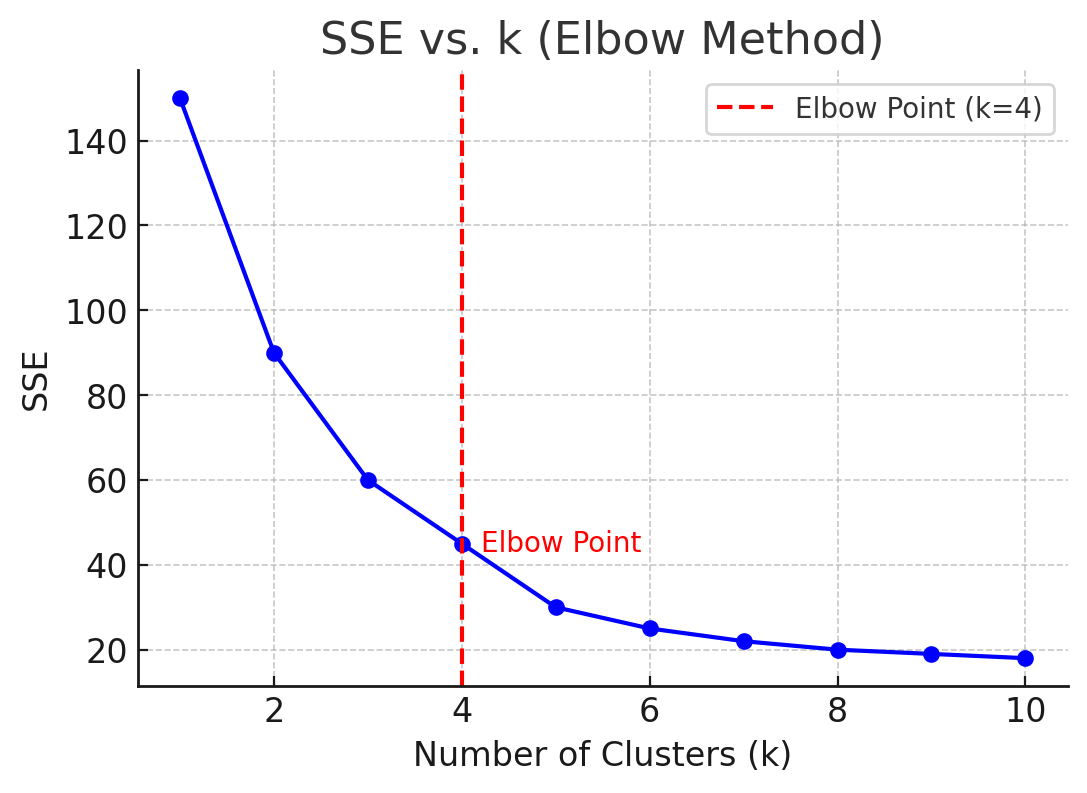
\includegraphics[width=0.45\linewidth]{ml/SSEkElbowmethod.png}
        \caption{An example of a graph showing SSE vs. $k$, and the elbow that can be used to pick the optimal $k$.}
        \label{fig:SSEkElbowmethod}
    \end{figure}

    Another method to determine \( k \) is by using the \textbf{silhouette score}, which evaluates how similar a data point is to its assigned cluster compared to other clusters. Higher silhouette scores indicate better-defined clusters.
\end{flushleft}

\subsection{Limitations of K-Means Clustering}
\begin{flushleft}
    \large While k-means is an effective clustering algorithm, it comes with several limitations:
    
    \begin{itemize}
        \item \textbf{Sensitivity to Initialization.} The algorithm is highly sensitive to the initial placement of the centroids. Poor initial choices can result in suboptimal clusters or even cause the algorithm to converge to a local minimum. To address this, a more refined initialization method, \textbf{K-Means++}, is often used to improve the initial centroids.
        
        \item \textbf{Fixed Number of Clusters.} K-means requires that \( k \) be defined ahead of time, which might not always be clear from the dataset. This adds complexity to its usage.
        
        \item \textbf{Sensitivity to Outliers.} K-means clustering can be significantly impacted by outliers. Since the algorithm seeks to minimize distances, outliers (data points far from the rest of the data) can disproportionately affect the cluster centroids.
    \end{itemize}
    
    Despite these limitations, k-means remains a widely used and powerful clustering technique for discovering patterns in data, particularly when the data is well-structured and the number of clusters is approximately known.
\end{flushleft}

\begin{questionbox}
\textbf{Synthesis Questions:}
\begin{enumerate}
    \item Define ``Unsupervised Learning'' and how it is different than ``Supervised Learning''.
    \item What is a centroid? How is it calculated?
    \item If the calculated centroids do not move very much after a few iterations, what does this indicate?
    \item If you have $n$ points to cluster, what value of $k$ will give the lowest SSE no matter how the points are formed? (\textbf{Hint:} It's kind of a cheap, degenerate case!)
    \item Why do you think k-means clustering is sensitive to centroid initialization?
\end{enumerate}
\end{questionbox}

\section{K-Means vs. K-Medians Clustering}
\subsection{Introduction to K-Medians Clustering}
\begin{flushleft}
    \large While \textbf{k-means} is a widely used method for clustering, an alternative approach is \textbf{k-medians clustering}, which offers a different way of calculating cluster centers. Instead of using the mean of the data points to define the cluster center as k-means does, k-medians calculates the center as the \textbf{median} of the data points in the cluster. This key difference makes k-medians more robust, particularly in the presence of \textbf{outliers}, as the median is less sensitive to extreme values.
    
    In k-medians, the objective is to minimize the sum of \textbf{absolute differences} between data points and the cluster center, rather than the sum of squared distances. This approach results in cluster centroids that are less influenced by anomalous data points, providing a more stable representation of the typical cluster member in datasets with noisy or skewed distributions.
\end{flushleft}

\subsection{K-Medians Use Cases}
\begin{flushleft}
    \large \textbf{K-medians} clustering is especially useful in situations where the data contains significant \textbf{outliers} or when using non-Euclidean distance metrics. Unlike k-means, which can be overly influenced by extreme values due to its reliance on the mean, k-medians offers a more \textbf{robust} solution by focusing on the median. For example, if a dataset contains several unusually large or small values that could distort the cluster centroid under k-means, k-medians will provide a more accurate and representative clustering result.

    K-medians is typically used when minimizing the \textbf{sum of absolute differences} between points is more meaningful than minimizing squared differences, such as in scenarios where data points vary widely in scale or when outliers are frequent. While k-medians may be less common than k-means in practice, it proves highly effective when the assumptions behind k-means (such as normal distribution of data or minimal outliers) do not hold.
\end{flushleft}

\subsection{Key Differences Between K-Means and K-Medians}
\begin{flushleft}
    \large The fundamental difference between \textbf{k-means} and \textbf{k-medians} lies in how they compute the cluster centroids and the distance metrics they use. K-means calculates the centroid as the \textbf{mean}, minimizing the sum of squared Euclidean distances. In contrast, k-medians uses the \textbf{median}, minimizing the sum of absolute distances (often referred to as Manhattan distance).

    Here are key distinctions between the two methods:
    
    \begin{itemize}
        \item \textbf{K-Means:} More sensitive to outliers because the mean is influenced by extreme values. It is best suited for datasets where the distance between points is naturally measured using Euclidean distances, and when the data does not contain many outliers.
        
        \item \textbf{K-Medians:} More robust to outliers, as the median remains stable even in the presence of extreme values. It is better suited for datasets with skewed distributions or where minimizing absolute differences is a priority.
    \end{itemize}

    \begin{figure}[H]
        \centering
        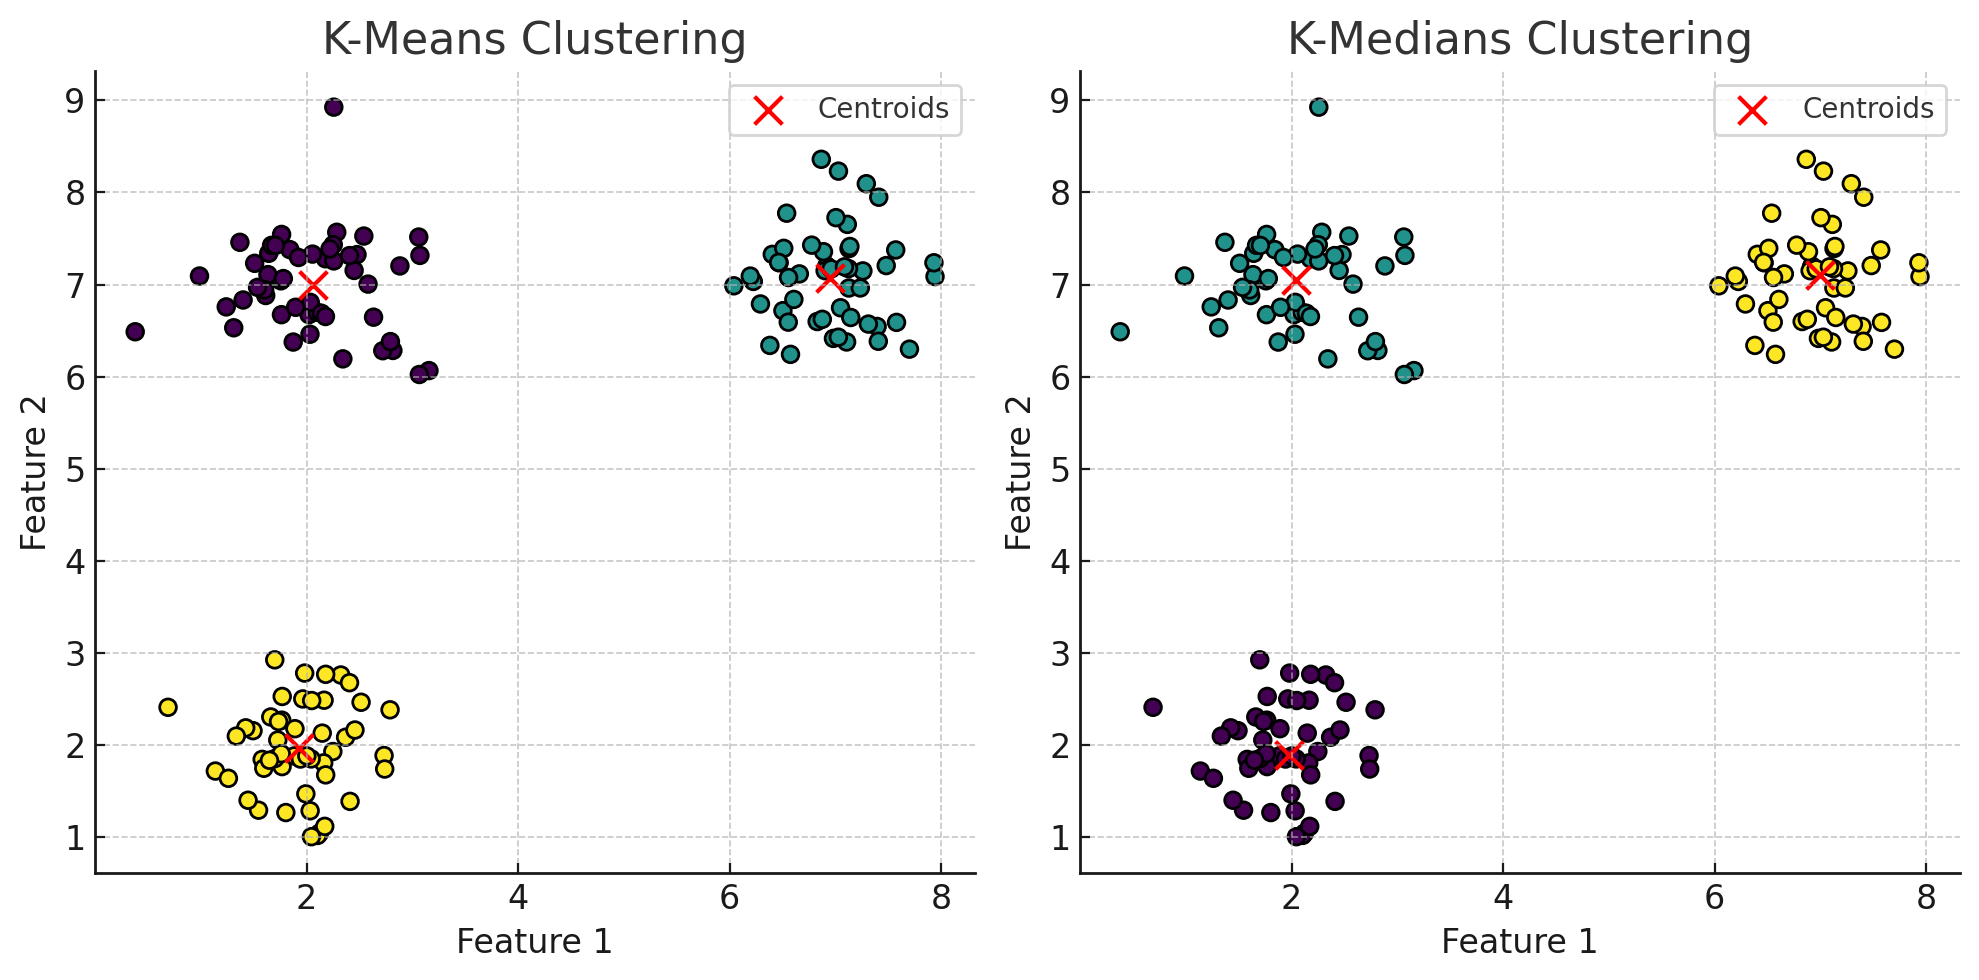
\includegraphics[width=0.45\linewidth]{ml/K-clustering.png}
        \caption{ An image comparing and contrasted the clusters created from k-means and k-medians methods.}
        \label{fig:K-clustering}
    \end{figure}
    
    The choice between the two methods depends heavily on the nature of the dataset. K-means is computationally more efficient but may produce distorted clusters in datasets with many outliers, whereas k-medians offers a more resilient solution for datasets with irregularities or noise.
\end{flushleft}

\begin{questionbox}
\textbf{Synthesis Questions:}
\begin{enumerate}
    \item Give a concrete, real-world example of a situation where \textit{k-means} clustering is a better choice than \textit{k-medians} clustering
    \item Give a concrete, real-world example of a situation where \textit{k-medians} clustering is a better choice than \textit{k-means} clustering
    \item Give a concrete, real-world example of a situation where \textit{neither} of these algorithms will work well
\end{enumerate}
\end{questionbox}

\section{Other ML Concepts}
\subsection{Bias-Variance Tradeoff}
\begin{flushleft}
    \large This is a concept that doesn't really fit anywhere else, but is incredibly important to talk about. The bias-variance tradeoff heavily rates to over and underfitting. \textbf{Overfitting} is when you have a model that fits the data it is trained on \textit{too} well. This could come about by, for example, trying to fit a very high-order polynomial curve to data that is linearly correlated. Instead of creating a line of best fit through the data, a sufficiently complex polynomial could just weave through every point in the graph. This would result in 0 SSE, but terrible performance on real-world data after the model is deployed. This is because real data is noisy, and a sufficiently complex model will fit to that noise because doing that technically minimizes SSE. \textbf{Underfitting} is the exact opposite problem. Say you had some synthetic data that took the shape of a parabola, but tried to fit a straight line to it. No matter how many training examples you provide, your model is not complex enough (you can also say it is not \textit{expressive} enough) to fit to the curve well. \break

    An example of a very basic, not-so-expressive linear model:

    $$y = w_1x_1 + b$$

    An example of a very expressive 5th-degree polynomial model:

    $$y = w_1x_1 + w_2x_1^2 + w_3x_1^3 + w_4x_1^4 + w_5x_1^5 + b$$

    A rarer, but still useful sinusoidal model:

    $$y = w_1\textrm{sin}(w_2x_1 - w_3) + b$$

    When people talk about the bias-variance tradeoff, they are essentially referring to over and under fitting, but are being a little more specific. \textbf{Bias} refers to how close the model line is to the ``true'' underlying curve. You can generate synthetic data for a line by generating points from some $y = mx +b$, but then adding a noise term $\epsilon \sim N(0, 1)$ to each point. If your underlying model fits to the generating $y = mx+b$ but ignores the noise introduced with $\epsilon$, then it has \textit{low bias}. \textbf{Variance} is a bit more complicated, but it essentially concerns the robustness of the model. If you were to add or remove a few points from a dataset, then a model with the appropriate level of expressivity should not change its learned coefficients by much. For example, if you had data correlating age with height, you shouldn't expect removing one or two points to affect the underlying correlation. A overly expressive model would, however, completely refit to swerve through all the points in a new way which drastically changes the coefficients. Variance measures how inconsistent the model is across different training subsets. When fitting ML models, you want a model that minimizes both bias \textit{and} variance. To do this, you must pick a ML model that has enough expressive power to capture underlying trends, but is not so expressive that it suffers from high variance errors. 

    \begin{figure}[H]
        \centering
        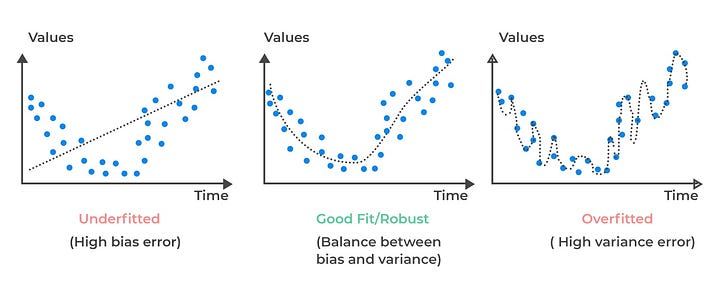
\includegraphics[width=0.8\linewidth]{ml/biasvariance.jpg}
        \caption{An illustration visualizing different balances between bias and variance for model fitting.}
        \label{fig:biasvariance}
    \end{figure}
\end{flushleft}

\subsection{Convexity}
\begin{flushleft}
    \large Convexity is important for ML models as well. So far, the linear models we have shown you are all \textbf{convex}. What this means is that we can guarantee we are able to converge upon an optimal set of weights if we train enough. You can think of optimizing a linear model like rolling down a valley. The lower you are on this valley, the lower the SSE. You take steps by fitting the model to training examples. Once you reach the bottom of this valley, you are satisfied as you cannot get any lower. Moving in any direction either increases your SSE or keeps it the same. \textit{If you are sure that the function you are optimizing is convex, then you can rest assured that you have found an optimal set of weights}. However, if the function you are optimizing on is non-convex, there is a chance that a lower valley exists somewhere on this SSE landscape, but you can never be 100\% certain!

    \begin{figure}[H]
        \centering
        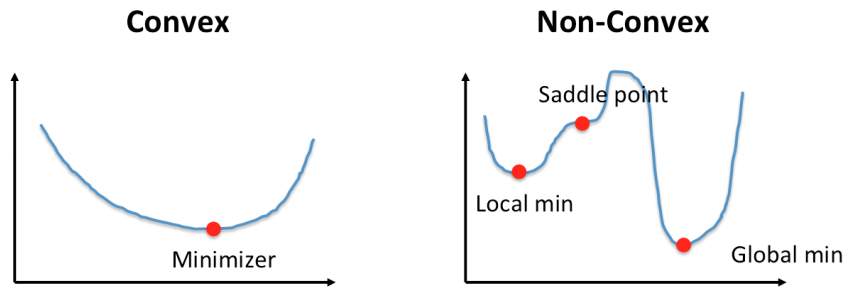
\includegraphics[width=0.8\linewidth]{ml/convexity.png}
        \caption{An illustration visualizing a convex function and a non-convex function. Also shown is the problem that comes with optimizing non-convex functions: getting stuck at a local minima.}
        \label{fig:convexity}
    \end{figure}
    
    Figure \ref{fig:convexity} illustrates this point. For the non-convex function, once you have reached a minimum, you don't know if it is a local minimum or a global minimum. However, in a convex function, you can be certain you have found a global minimum. Knowing that you are working with a convex optimization problem (i.e. a linear model) gives you the peace of mind in knowing that with enough training you will find weights that fit the data as well as possible for the model's complexity class.
\end{flushleft}

\begin{questionbox}
\textbf{Synthesis Questions:}
\begin{enumerate}
    \item What does ``expressivity''  of a function mean?
    \item How do over and underfitting relate to bias and variance?
    \item If a model gives low bias and variance while fitting to a dataset, is it a good choice?
    \item Why is knowing that your optimization problem is convex useful/good?
    \item \textbf{Bonus:} Are either k-means or k-medians convex optimization problems? Give reasoning (does not need to be in proof form)
\end{enumerate}
\end{questionbox}

\section{When to Use Machine Learning Algorithms}
\begin{flushleft}
    \large Machine learning models are widely used in applications like image recognition, natural language processing, and predictive analytics. However, selecting the right algorithm for a task is essential. Simple models like linear regression may suffice for tasks with linear relationships, while more complex tasks (like image classification) often require more advanced models, such as neural networks. \break
    
    Furthermore, unsupervised learning methods like k-means clustering are valuable when you want to find hidden patterns in the data without labeled outcomes. \break
\end{flushleft}

\section{Conclusion (ML)}
\begin{flushleft}
    \large This section covered the fundamental concepts of machine learning, with a focus on supervised learning (linear regression) and unsupervised learning (k-means clustering). We also introduced important concepts like regularization (L1 and L2), the bias-variance tradeoff, and convexity. Additionally, we discussed the differences between k-means and k-medians clustering and clarified why logistic regression is a classification algorithm. Understanding these basics is crucial as machine learning continues to influence more of our lives. These concepts are also the most applicable in day-to-day ML, the backbone of modern systems. More often than not, Occam's Razor holds true: Don't use more than necessary and overcomplicate things. \break
\end{flushleft}
